\documentclass[letterpaper]{article}
\usepackage[square,sort,comma,numbers]{natbib}
\usepackage{array}
%====================================================================%
../../../../tex/scufftex.tex
\graphicspath{{figures/}}
\renewcommand{\wt}{\widetilde}
\newcommand{\vbCSlash}{\backslash\hspace{-0.085in}\vb C}
\newcommand{\JSlash}{\backslash\hspace{-0.085in}J}

%------------------------------------------------------------
%------------------------------------------------------------
%- Special commands for this document -----------------------
%------------------------------------------------------------
%------------------------------------------------------------

%------------------------------------------------------------
%------------------------------------------------------------
%- Document header  -----------------------------------------
%------------------------------------------------------------
%------------------------------------------------------------
\title {Implicit handling of multilayered material substrates
        in full-wave {\sc scuff-em} calculations
       }
\author {Homer Reid}
\date {August 16, 2017}

%------------------------------------------------------------
%------------------------------------------------------------
%- Start of actual document
%------------------------------------------------------------
%------------------------------------------------------------

\begin{document}
\pagestyle{myheadings}
\markright{Homer Reid: Implicit substrates in full-wave {\sc scuff-em}}

\maketitle

\tableofcontents

%====================================================================%
%====================================================================%
%====================================================================%
\newpage
\section{Overview}

In a 
previous memo\footnote{``Implicit handling of multilayered dielectric
substrates in {\sc scuff-static}''} I
considered {\sc scuff-static} electrostatics calculations
in the presence of a multilayered dielectric substrate.
In this memo I extend that discussion to the case of
\textit{full-wave} (i.e. nonzero frequencies beyond the
quasistatic regime) scattering calculations in the
{\sc scuff-em} core library.

%%%%%%%%%%%%%%%%%%%%%%%%%%%%%%%%%%%%%%%%%%%%%%%%%%%%%%%%%%%%%%%%%%%%%%
%%%%%%%%%%%%%%%%%%%%%%%%%%%%%%%%%%%%%%%%%%%%%%%%%%%%%%%%%%%%%%%%%%%%%%
%%%%%%%%%%%%%%%%%%%%%%%%%%%%%%%%%%%%%%%%%%%%%%%%%%%%%%%%%%%%%%%%%%%%%%
\subsubsection*{Substrate geometry}

As shown in Figure \ref{SubstrateGeometryFigure}, I consider
a multilayered substrate consisting of $N$ material layers
possibly terminated by a perfectly-conducting ground plane.
The uppermost layer (layer 1) is the infinite half-space
above the substrate.
The $n$th layer
has relative permittivity and permeability $\epsilon_n,\mu_n$,
and its lower surface lies at $z=z_n$.
The ground plane, if present,
lies at $z\equiv z\subt{N}\equiv z\subt{GP}$.
If the ground plane is absent, layer $N$ is an
infinite half-space\footnote{As in the electrostatic case,
this means that a finite-thickness substrate consisting of
$N$ material layers is described as a stack of $N+1$ layers
in which the bottommost layer is an infinite vacuum half-space.}
($z\subt{N}=-\infty$).
%####################################################################%
%####################################################################%
%####################################################################%
\begin{figure}[!]
\begin{center}
\resizebox{\textwidth}{!}{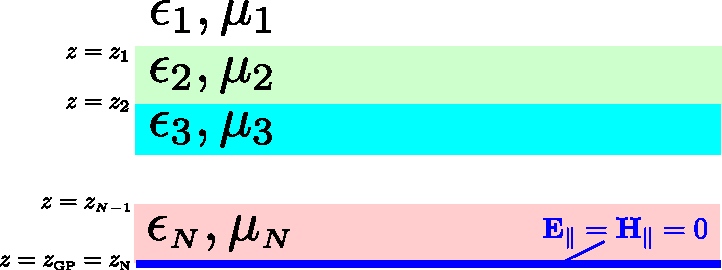
\includegraphics{MultilayerSubstrate.pdf}}
\caption{Geometry of the layered substrate.
The $n$th layer 
has relative permittivity and permeability $\epsilon_n,\mu_n$,
and its lower surface lies at $z=z_n$. The ground plane, if present,
lies at $z=z\subt{GP}.$
}
\label{SubstrateGeometryFigure}
\end{center}
\end{figure}
%####################################################################%

%%%%%%%%%%%%%%%%%%%%%%%%%%%%%%%%%%%%%%%%%%%%%%%%%%%%%%%%%%%%%%%%%%%%%%
%%%%%%%%%%%%%%%%%%%%%%%%%%%%%%%%%%%%%%%%%%%%%%%%%%%%%%%%%%%%%%%%%%%%%%
%%%%%%%%%%%%%%%%%%%%%%%%%%%%%%%%%%%%%%%%%%%%%%%%%%%%%%%%%%%%%%%%%%%%%%
\subsubsection*{Definition of the substrate DGF}

For given source and evaluation (or ``destination'')
points $\{\vb x\subt{S}, \vb x\subt{D}\}$ at a given angular frequency
$\omega$ in the presence of a multilayer substrate,
the $\vb E$ and $\vb H$ fields at $\vb x\subt{D}$ due to 
point sources at $\vb x\subt{S}$ receive corrections (relative
to their free-space values) due to the presence of the
substrate. These are described by the substrate dyadic Green's 
function $\bmc G(\omega; \vb x\subt{D}, \vb x\subt{S}),$ a
$6\times 6$ matrix with a $2\times 2$ block structure:
%====================================================================%
\begin{subequations}
\begin{align} 
 \bmc G(\omega; \vb x\subt{D}, \vb x\subt{S})
&=
 \left(\begin{array}{cc}
   \bmc G\supt{EE} & \bmc G\supt{EM} \\
   \bmc G\supt{ME} & \bmc G\supt{MM}
 \end{array}\right)
\intertext{with the $3\times 3$ subblocks defined by} 
\mc G\supt{PQ}_{ij}&=
\left(\begin{parbox}{0.6\textwidth}
  { substrate contribution to $i$-component of 
    P-type field at $\vb x\subt{D}$ due to 
    $j$-directed Q-type source at $\vb x\subt{S}$
    with angular frequency $\omega$
  } \end{parbox}\right)
\end{align}
\label{ScriptGDef}%
\end{subequations}
%====================================================================%
Iff $\vb x\subt{S}, \vb x\subt{D}$ lie in the same layer of the multilayer
substrate, then to get the \textit{total} fields
(\ref{ScriptGDef}) must be augmented by the contribution
of the homogeneous DGF of the medium::
%====================================================================%
\numeq{GTotal}
{
 \bmc G\sups{total}(\omega, \vb x\subt{S}, \vb x\subt{D})
=
 \left(\begin{array}{cc}
   \bmc G\supt{EE} & \bmc G\supt{EM} \\
   \bmc G\supt{ME} & \bmc G\supt{MM}
 \end{array}\right)
  +
 \left(\begin{array}{cc}
   ik_r Z_0 Z^r \vb G & ik_r \vb C           \\
  -ik_r \vb C & \frac{ik_r}{Z_0 Z^r} \vb C \\
 \end{array}\right),
 \quad \vb x\subt{S}, \vb x\subt{D} \in \text{layer \#$r$}
}
where $k_r, Z^r$ are the wavevector and relative wave impedance
of substrate layer $r$.
%====================================================================%
On the other hand, if $\vb x\subt{S}, \vb x\subt{D}$ lie in different
layers then $\bmc G$ in (\ref{ScriptGDef}) already gives
the total field at $\vb x\subt{D}$.

%%%%%%%%%%%%%%%%%%%%%%%%%%%%%%%%%%%%%%%%%%%%%%%%%%%%%%%%%%%%%%%%%%%%%%
%%%%%%%%%%%%%%%%%%%%%%%%%%%%%%%%%%%%%%%%%%%%%%%%%%%%%%%%%%%%%%%%%%%%%%
%%%%%%%%%%%%%%%%%%%%%%%%%%%%%%%%%%%%%%%%%%%%%%%%%%%%%%%%%%%%%%%%%%%%%%
\subsubsection*{Organization of {\sc scuff-em} implementation and this memo}

The full-wave substrate implementation in {\sc scuff-em} consists of
multiple working parts that fit together in a somewhat modular fashion.

Roughly speaking, the computational problem may be divided into two parts:
%====================================================================%
\begin{description}
  \item[(a)] For given source and evaluation (or ``destination'')
             points $\{\vb x\subt{S}, \vb x\subt{D}\}$ at a given 
             angular frequency
             $\omega$ in the presence of a multilayer substrate,
             numerically compute the substrate DGF correction
             $\bmc G(\omega, \vb x\subt{D}, \vb x\subt{S})$.
             This task is independent of {\sc scuff-em}
             and is implemented by a standalone library
             called {\sc libsubstrate}, described in
             Section \ref{libSubstrateSection} of this memo.
  \item[(b)] For a {\sc scuff-em} geometry in the presence of a
             substrate, compute the substrate corrections to the BEM
             system matrix $\vb M$ and RHS vector $\vb v$,
             as well as the substrate corrections
             to post-processing quantities such as scattered fields.
             This is done by the file \texttt{Substrate.cc}
             in {\sc libscuff} and is described in 
             Section \ref{libscuffIntegrationSection} of this memo.
\end{description}
%====================================================================%

%####################################################################%
%####################################################################%
%####################################################################% 
\newpage
\section{{\sc libsubstrate:} Numerical computation of substrate Green's functions}
\label{libSubstrateSection}

Numerical evaluation of substrate contributions to
dyadic Green's functions is handled by a C++ library 
called {\sc libsubstrate}.
Although this library is packaged and distributed with {\sc scuff-em}
and depends on other support libraries in the {\sc scuff-em}
distribution, it is independent of the particular integral-equation
formulation implemented by {\sc libscuff}, and thus should be
of general utility beyond {\sc scuff-em}.

\subsection{Overview of computational strategy}
\label{libSubstrateStrategy}

{\sc libsubstrate} decomposes the problem of computing
$\bmc G$ into several logical steps, as follows:

\begin{description}
 \item[1.] Solve a linear system to obtain the Fourier-space
             representation $\bmc{\wt G(\vb q)}$. Here $\vb q=(q_x,q_y)$ is a
             2D Fourier variable. (Section \ref{GTwiddleSection}.)
 \item[2.] Reduce the two-dimensional integral over $\vb q$ to a
             one-dimensional integral over $|\vb q|\equiv q$.
             (Section \ref{gTwiddleSection}.)
 \item[3.] Evaluate the $q$ integral using established methods for
             evaluating Sommerfeld integrals.
             (Section \ref{SommerfeldSection}.)
\end{description}

%%%%%%%%%%%%%%%%%%%%%%%%%%%%%%%%%%%%%%%%%%%%%%%%%%%%%%%%%%%%%%%%%%%%%%
%%%%%%%%%%%%%%%%%%%%%%%%%%%%%%%%%%%%%%%%%%%%%%%%%%%%%%%%%%%%%%%%%%%%%%
%%%%%%%%%%%%%%%%%%%%%%%%%%%%%%%%%%%%%%%%%%%%%%%%%%%%%%%%%%%%%%%%%%%%%%
\newpage
\subsection{Computation of Fourier-space DGF $\bmc{\wt G}(\vb q)$}
\label{GTwiddleSection}

%####################################################################%
%####################################################################%
%####################################################################%
\begin{figure}[t]
\begin{center}
\resizebox{\textwidth}{!}{\includegraphics{MultilayerSubstrateWithSurfaceCurrents.pdf}}
\caption{Effective surface-current approach to treatment of
multilayer substrate. External field sources induce a distribution
of electric and magnetic surface currents $\bmc S_n={\vb K_n \choose \vb N_n}$
on the $n$th material interface, and the fields radiated by these
effective currents account for the disturbance presented by
the substrate.}
\label{SurfaceCurrentFigure}
\end{center}
\end{figure}
%####################################################################%
%####################################################################%
%####################################################################%
To compute the substrate correction to the fields of external sources,
I consider the effective tangential electric and magnetic
surface currents $\vb K$ and $\vb N$ induced on the interfacial 
layers by the external field sources 
(Figure \ref{SurfaceCurrentFigure}). This is the direct extension
to full-wave problems of the formalism I used in the electrostatic
case, and it comports well with the spirit of
surface-integral-equation methods.

More specifically, on the material interface layer at $z=z_n$
I have a four-vector surface-current density $\bmc S_n(\vbrho)$,
where $\vbrho=(x,y)$ and the components of $\bmc S$ are
%====================================================================%
\numeq{SnDef}
{ \bmc S_n(\vbrho)=
  \left(\begin{array}{c}
     K_x(\vbrho) \\ K_y(\vbrho) \\ N_x(\vbrho) \\ N_y(\vbrho)
  \end{array}\right).
}
%====================================================================%

\paragraph{Fields in layer interiors.} 
I will adopt the convention that the lower (upper) bounding surface
for each region is the positive (negative) bounding surface
for that region in the usual sense of {\sc scuff-em} regions and
surfaces (in which the sign of a \{surface,region\} pair $\{\mc S, \mc R\}$ 
is the sign with which surface currents on $\mc S$ contribute to
fields in $\mc R$).
Thus, at a point $\vb x=(\vbrho,z)$ in the interior of layer $n$
($z_{n-1} > z > z_n$), the six-vector of total fields
$\bmc F=\hbox{\scriptsize{
 $\left(\begin{array}{c} \vb E \\ \vb H\end{array}\right)$}}
$
reads
%====================================================================%
\numeq{Fn}
{  \bmc F_n(\vbrho, z)
  =
  - \bmc G^{0n}(z_{n-1}) \star \bmc S_{n-1}
  + \bmc G^{0n}(z_{n}) \star \bmc S_{n}
  + \bmc F\sups{ext}_n(\vbrho, z)
}
%====================================================================%
where $\bmc F\sups{ext}_n$
are the externally-sourced (incident) fields
due to sources in layer $n$, $\bmc G^{0n}$ is the homogeneous dyadic
Green's function for material layer $n$, and $\star$
is shorthand for the convolution operation
%====================================================================%
\numeq{ConvolutionDef}
{
``\bmc F(\vbrho, z) \equiv \bmc G(z^\prime) \star \bmc S''
   \quad \Longrightarrow \quad 
    \bmc F(\vbrho,z) = 
    \int
      \bmc G(\vbrho-\vbrho^\prime,z-z^\prime)\cdot \bmc S(\vbrho^\prime)
    d\vbrho^\prime
}
%====================================================================%
where the integral extends over the entire interfacial plane.
I will evaluate convolutions of this form using the
2D Fourier representation of $\bmc G^{0n}$:
%====================================================================%
\begin{subequations}
\begin{align}
  \bmc G^{0n}(\vbrho, z)
 &=
  \int \frac{d^2 \vb q}{(2\pi)^2}
  \wt{\bmc G^{0n}}(\vb q, z) e^{i\vb q \cdot \vbrho}
\\
%--------------------------------------------------------------------%
   \wt{\bmc G^{0n}}(\vb q, z)
&= \frac{1}{2}
   \left(\begin{array}{cc}
      -\frac{\omega \mu_0 \mu_n}{q_{zn}} \wt{\vb G}^\pm
    & +\wt{\vb C}^\pm 
    \\[5pt]
      -\wt{\vb C}^\pm
    & -\frac{\omega \epsilon_0 \epsilon_n}{q_{zn}} \wt{\vb G}^\pm
   \end{array}\right)e^{iq_z |z|}
\\[10pt]
%--------------------------------------------------------------------%
   \wt{\vb G}^\pm(\vb q, k)
&= \left(\begin{array}{ccc}
   1 & 0 & 0 \\[2pt] 0 & 1 & 0 \\[2pt] 0 & 0 & 1
   \end{array}\right)
   -
   \frac{1}{k^2}
   \left(\begin{array}{ccc}
    q_x^2    & q_xq_y       & \pm q_x q_z \\[2pt]
    q_y q_x  & q_y^2        & \pm q_y q_z \\[2pt]
 \pm q_z q_x  & \pm q_z q_y  & q_z^2 
   \end{array}\right)
\\[10pt]
%--------------------------------------------------------------------%
   \wt{\vb C}^\pm(\vb q, k)
&=
   \left(\begin{array}{ccc}
   0           & \mp 1     &    +q_y/q_z \\[2pt]
   \pm 1       & 0         &    -q_x/q_z \\[2pt]
  -q_y/q_z     & +q_x/q_z  &           0
  \end{array}\right)
\end{align}
\label{GFourier}
\begin{equation}
  k_n\equiv \sqrt{\epsilon_0 \epsilon_n \mu_0 \mu_n}\cdot \omega,
  \qquad 
  q_z \equiv \sqrt{k^2 - |\vb q|^2},
 \qquad 
  \pm = \text{sign } z.
\end{equation}
\end{subequations}
%====================================================================%
\noindent With this representation, convolutions like (\ref{ConvolutionDef})
become products in Fourier space:
%====================================================================%
\begin{align*}
\bmc G(z^\prime)\star \bmc S=
 \bmc F(\vbrho, z)
&=\int \frac{d^2 \vb q}{(2 \pi)^2} \wt{\bmc F}(\vb q,z) e^{i\vb q \cdot \vbrho},
\qtq{with}
 \wt{\bmc F(\vb q,z)}=\wt{\bmc G}(\vb q,z-z^\prime)\wt{\bmc S}(\vb q)
\end{align*}
%====================================================================%

\paragraph{Surface currents from incident fields.}

To determine the surface currents induced by given incident-field
sources, I apply boundary conditions.
The boundary condition at $z=z_n$ is that the tangential $\vb E, \vb H$
fields be continuous: in Fourier space, we have
%====================================================================%
\numeq{BCEquation}
{ \wt{\bmc F}_{\parallel}(\vb q, z=z_n^+)
 =\wt{\bmc F}_{\parallel}(\vb q, z=z_n^-)
}
The fields just \textbf{above} the interface $(z\to z_n^+)$ receive
contributions from three sources:
%====================================================================%
\begin{itemize}
 \item Surface currents at $z=z_{n-1}$, which contribute with
       a minus sign and via the Green's function for region $n$;
 \item Surface currents at $z=z_{n}$, which contribute with
       a plus sign and via the Green's function for region $n$; and
 \item external field sources in region $n$.
\end{itemize}
%====================================================================%
The fields just \textbf{below} the interface $(z=z_n^-)$ receive
contributions from three sources:
%====================================================================%
\begin{itemize}
 \item Surface currents at $z=z_{n}$, which contribute with
       a minus sign and via the Green's function for region $n+1$;
 \item Surface currents at $z=z_{n+1}$, which contribute with
       a plus sign and via the Green's function for region $n+1$; and
 \item external field sources in region $n+1$.
\end{itemize}
%====================================================================%
Then equation (\ref{BCEquation}) reads
%====================================================================%
\begin{align*}
&
-\wt{\bmc G^{0n}}_{\parallel}(z_n-z_{n-1})\cdot \wt{\bmc S}_{n-1}
+\wt{\bmc G^{0n}}_{\parallel}(0^+) \cdot \wt{\bmc S}_{n}
+\wt{\bmc F}\sups{ext}_{n\parallel}(z_n)
\\
&\qquad=
-\wt{\bmc G^{0,n+1}}{\parallel}(0^-) \cdot \wt{\bmc S}_{n}
+\wt{\bmc G^{0,n+1}}{\parallel}(z_n-z_{n+1})\cdot \wt{\bmc S}_{n+1}
+\wt{\bmc F}\sups{ext}_{n+1\parallel}(z_n)
\end{align*}
or
%====================================================================%
\numeq{MSFSlice}
{
  \vb M_{n,n-1}  \cdot \wt{\bmc S}_{n-1}
 +\vb M_{n,n}    \cdot \wt{\bmc S}_{n}
 +\vb M_{n,n+1}  \cdot \wt{\bmc S}_{n+1}
 =  \wt{\bmc F}\sups{ext}_{n+1\parallel}(z_n)
   -\wt{\bmc F}\sups{ext}_{n\parallel}(z_n)
}
%====================================================================%
with the $4\times 4$ matrix blocks\footnote{The $4\times 4$ $\vb M$
blocks here have $2\times 2$ block structure:
%====================================================================%
\begin{align}
 \vb M_{n, n}
   &= \sum_{r\in \{n, n+1\}}
     \frac{1}{2}
     \left(\begin{array}{cc}
     -\frac{\omega\epsilon_r}{Z_0 q_{zr}}\vb g(k_r, \vb q)
   & 0
 \\
     0
   & -\frac{\omega\mu_r Z_0 }{q_{zr}}\vb g(k_r, \vb q)
   \end{array}\right)
\\
 \vb M_{n, n \pm 1}
   &= \frac{1}{2}
     \left(\begin{array}{cc}
     -\frac{\omega\epsilon_r}{Z_0 q_{zr}}\vb g(k_r, \vb q)
   & \vb c^\pm
 \\
     -\vb  c^\pm
   & -\frac{\omega\mu_r Z_0 }{q_{zn^*}}\vb g(k_r, \vb q)
     \end{array}\right)e^{iq_{zr}|z_n-z_{n\pm 1}|}
\end{align}
%====================================================================%
where I put
$  r \equiv  \begin{cases} n,   \qquad &\text{ for } \vb M_{n,n-1} \\
                           n+1, \qquad &\text{ for } \vb M_{n,n+1}
              \end{cases}.
$
and 
%====================================================================%
$$ \vb g(k; \vb q) =
   \vb 1 - \frac{\vb q\vb q^\dagger}{k^2},
   \qquad 
   \vb c^\pm
   =\left(\begin{array}{cc} 0 & \mp 1 \\ \pm 1 & 0 \end{array}\right)
$$}
%====================================================================%
%====================================================================%
\begin{subequations}
\begin{align}
  \vb M_{n,n-1} &= -\wt{\bmc G^{0n}}_{\parallel}(z_n-z_{n-1}) 
\\
  \vb M_{n,n} &= +\wt{\bmc G^{0n}}_{\parallel}(0^+)
                 +\wt{\bmc G^{0,n+1}}_{\parallel}(0^-)
\\
  \vb M_{n,n+1} &= -\wt{\bmc G^{0,n+1}}_{\parallel}(z_n-z_{n+1}) 
\end{align}
\label{MChunks}
\end{subequations}
%====================================================================%
Writing down equation (\ref{MSFSlice}) equation for all $N$ dielectric
interfaces yields a $4N\times 4N$ 
system of linear equations, with triadiagonal $4\times 4$ block form,
relating the surface currents on all layers
to the external fields due to sources in all regions:
%====================================================================%
\numeq{Msf}{\vb M\cdot \vb s = \vb f}
%====================================================================%
where $\vb M$ is the $4N\times 4N$ block-tridiagonal matrix
(\ref{MChunks}) and where the $4N$-vectors $\vb s$, $\vb f$ read
%====================================================================%
$$ 
   \vb s=\left(\begin{array}{c}
   \wt{\bmc S}_1 \\ \wt{\bmc S}_2 \\ \wt{\bmc S}_3 \\ \vdots \\
   \wt{\bmc S}_N
   \end{array}\right),
\qquad 
   \vb f=\left(\begin{array}{c}
  -\wt{\bmc F}_{1\parallel}(z_1)
  +\wt{\bmc F}_{2\parallel}(z_1)
\\
  -\wt{\bmc F}_{2\parallel}(z_2)
  +\wt{\bmc F}_{3\parallel}(z_2)
\\
  -\wt{\bmc F}_{3\parallel}(z_3)
  +\wt{\bmc F}_{3\parallel}(z_4)
\\
  \vdots
\\
  -\wt{\bmc F}_{N-1,\parallel}(z_{N-1})
  +\wt{\bmc F}_{N\parallel}(z_{N-1})
   \end{array}\right).
$$
%====================================================================%
Solving (\ref{Msf}) yields the induced surface currents on all
layers in terms of the incident fields:
%====================================================================%
$$ \vb s = \vb W \cdot \vb f \qtq{where} \vb W\equiv \vb M^{-1} $$
%====================================================================%
or, more explicitly,
%====================================================================%
\numeq{sWf}
{
 \wt{\bmc S}_n = \sum_{m} W_{nm} \vb f_m
}
%====================================================================%

%====================================================================%
%====================================================================%
%====================================================================%
\subsubsection*{Surface currents induced by point sources}

For DGF computations the incident fields arise from
a single point source---say, a $j$-directed source
in region $s$.
Then the only nonzero length-$4$ blocks of the RHS vector in
(\ref{Msf}) are $\vb f_{s-1}, \vb f\subt{S}$ with components
($\ell=\{1,2,4,5\}$)
%====================================================================%
\numeq{fsm1fs}
 { \Big(\vb f_{s-1}\Big)_\ell = -\wt{\mc G}_{\ell j}^{0s}( z_{s-1}-z\subt{S}),
   \qquad
   \Big(\vb f_{s}\Big)_\ell   = +\wt{\mc G}_{\ell j}^{0s}(z\subt{S}-z\subt{S})
 }
%====================================================================%
and the surface currents on interface layer $n$ are obtained
by solving (\ref{sWf}):
%====================================================================%
\begin{align}
 \wt{\bmc S}_n 
&= \vb W_{n,s-1} \, \vb f_{s-1} + \vb W_{n,s} \, \vb f_{s}
\nn
&= \sum_{p=0}^1 (-1)^{p+1} \vb W_{n,s-1+p}
    \cdot
    \wt{\bmc G^{0s}}_{\parallel, j}(z\subt{S}-z_{s-1+p})
\label{SWG}
\end{align}
%====================================================================%

%====================================================================%
%====================================================================%
%====================================================================%
\subsubsection*{Fields due to surface currents}

Given the surface currents induced by a $j$-directed point
source at $\vb x\subt{S}$, I evaluate the fields due to
these currents to get DGF components.
If the evaluation point $\vb x\subt{D}$ lies in region $d$,
then the fields receive contributions from the surface currents
at $z_{d-1}$ and $z\subt{D}$, propagated by the homogeneous DGF
for region $d$:
%====================================================================%
\begin{align}
\wt{\bmc F}(z\subt{D}) 
&= -\wt{\bmc G^{0d}}(z\subt{D} - z_{d-1}) \cdot \wt{\bmc S}_{d-1}
   +\wt{\bmc G^{0d}}(z\subt{D} - z\subt{D})     \cdot \wt{\bmc S}_{d}
\nn
&= \sum_{q=0}^1  (-1)^{q+1}
   \wt{\bmc G^{0d}}(z\subt{D} - z_{d+q-1}) \cdot \wt{\bmc S}_{d+q-1}
\nonumber
\intertext{(The minus sign in the first term arises because, in my convention,
surface currents on the upper surface of a region contribute to the fields
in that region with a minus sign). Inserting (\ref{SWG}), the $i$ component
here---which is the $ij$ component of the substrate DGF---is}
\wt{\mc G}_{ij}(z\subt{D},z\subt{S})
\equiv
\wt{\mc F_i}(z\subt{D})
&= \sum_{p,q=0}^1 (-1)^{p+q}
   \wt{\bmc G^{0d}}_{i,\parallel} (z\subt{D}-z_{d-1+q})
   \vb W_{d-1+q,s-1+p}
   \wt{\bmc G^{0s}}_{\parallel, j} (z_{s-1+p} - z\subt{S})
\label{ScriptGFourier}
\end{align}
%====================================================================%

%%%%%%%%%%%%%%%%%%%%%%%%%%%%%%%%%%%%%%%%%%%%%%%%%%%%%%%%%%%%%%%%%%%%%%
%%%%%%%%%%%%%%%%%%%%%%%%%%%%%%%%%%%%%%%%%%%%%%%%%%%%%%%%%%%%%%%%%%%%%%
%%%%%%%%%%%%%%%%%%%%%%%%%%%%%%%%%%%%%%%%%%%%%%%%%%%%%%%%%%%%%%%%%%%%%%
\newpage
\subsection{Reduction of 2D integrals over $\vb q$ to 1D (Sommerfeld) integrals over $q$}
\label{gTwiddleSection}

The real-space DGF is the inverse Fourier transform of 
(\ref{ScriptGFourier}):
%====================================================================%
\numeq{IFT2D}
{
  \bmc G(\vbrho\subt{D}, z\subt{D}; \vbrho\subt{S},z\subt{S})
= \int \frac{d^2 \vb q}{(2\pi)^2}
  \wt{\bmc G}
      (\vb q; z\subt{D};z\subt{S}) e^{i\vb q \cdot (\vbrho \subt{D}-\vbrho\subt{S})}.
}
%====================================================================%
I will evaluate the $\vb q$ integral here in polar coordinates, 
$\vb q=(q_x,q_y)=\big(q \cos\theta_{\vb q}, q\sin\theta_{\vb q}\big)$
with $q=|\vb q|$.
Although $\wt{G}(\vb q)$ has 36 Cartesian components,
these may be expressed in terms of just 18 scalar functions
of $q$ times cosines and sines of $\theta_{\vb q}$:
%====================================================================%
\begin{align*}
 \wt{\bmc G\supt{EE}}(\vb q)
 = &\wt{g}\supt{EE0$\parallel$}(q)
    \underbrace{ \left(\begin{array}{ccc}
                       1 & 0 & 0 \\ 
                       0 & 1 & 0 \\ 
                       0 & 0 & 0 \\ 
                 \end{array}\right)
               }_{\vbLambda^{0\parallel}}
  + \wt{g}\supt{EE0$z$}(q)
    \underbrace{ \left(\begin{array}{ccc}
                       0 & 0 & 0 \\ 
                       0 & 0 & 0 \\ 
                       0 & 0 & 1 \\ 
                 \end{array}\right)
               }_{\vbLambda^{0z}}
\\[10pt]
%--------------------------------------------------------------------%
 + &\wt{g}\supt{EE1A}(q)
    \underbrace{ \left(\begin{array}{ccc}
                       0 & 0 & \cos\theta_{\vb q} \\ 
                       0 & 0 & \sin\theta_{\vb q} \\ 
                       0 & 0 & 0 \\ 
                 \end{array}\right)
               }_{\vbLambda^{1}(\theta_{\vb q})}
 +  \wt{g}\supt{EE1B}(q)
    \underbrace{ \left(\begin{array}{ccc}
                       0 & 0 & 0 \\
                       0 & 0 & 0 \\
                       \cos\theta_{\vb q} & \sin\theta_{\vb q} & 0
                 \end{array}\right)
               }_{\vbLambda^{1\dagger}(\theta_{\vb q})}
\\[10pt]
%--------------------------------------------------------------------%
  +&\wt{g}\supt{EE2}(q)
    \underbrace{
   \left(\begin{array}{ccc}
    \cos^2\theta_{\vb q}  & \cos\theta_{\vb q} \sin\theta_{\vb q} & 0 \\
    \cos\theta_{\vb q} \sin\theta_{\vb q} & \sin^2\theta_{\vb q}  & 0 \\
    0                     & 0                    & 0 
   \end{array}\right)
               }_{\vbLambda^{2A}(\theta_{\vb q})}
\\[20pt]
%--------------------------------------------------------------------%
 \wt{\bmc G\supt{EM}}(\vb q)
 = &g\supt{EM0$\parallel$}(q)
    \underbrace{ \left(\begin{array}{ccc}
                       0 & 1 & 0 \\ 
                      -1 & 0 & 0 \\ 
                       0 & 0 & 0 
                 \end{array}\right)
               }_{\vbLambda^{0\times}}
  +g\supt{EM2}(q)
   \underbrace{
   \left(\begin{array}{ccc}
    \cos\theta_{\vb q} \sin\theta_{\vb q} & \sin^2\theta_{\vb q} & 0 \\
    -\cos^2\theta_{\vb q} & -\cos\theta_{\vb q} \sin\theta_{\vb q} & 0 \\
    0                     & 0                    & 0 
   \end{array}\right)
              }_{\vbLambda^{2\times}}
\\[10pt]
%--------------------------------------------------------------------%
  + &g\supt{EM1A}(q)
   \underbrace{
    \left(\begin{array}{ccc}
    0 & 0 & -\sin\theta_{\vb q} \\
    0 & 0 & +\cos\theta_{\vb q} \\
    0 & 0 & 1
   \end{array}\right)
              }_{\vbLambda^{1\times}}
  + g\supt{EM1B}(q)
   \underbrace{
    \left(\begin{array}{ccc}
    0 & 0 & 0 \\
    0 & 0 & 0 \\
   -\sin\theta_{\vb q} & \cos\theta_{\vb q} & 1
   \end{array}\right)
              }_{\vbLambda^{1\times\dagger}}
\end{align*}
(The expressions for $\wt{\bmc G}\supt{ME}$ and $\wt{\bmc G}\supt{MM}$ are
similar.)
%====================================================================%
\begin{align*}
 \int \frac{d \vb q}{(2\pi)^2} \wt g(q) e^{i\vb q \cdot \vbrho} \vbLambda^{(0)}
&=\int \frac{qdq}{2\pi} \wt g(q) J_0(q\rho) \vbLambda^{(0)}
\\
 \int \frac{d \vb q}{(2\pi)^2} \wt g(q) e^{i\vb q \cdot \vbrho} \vbLambda^{(1)}(\theta_{\vb q})
&=i\int \frac{qdq}{2\pi} \wt g(q) J_1(q\rho) \vbLambda^{(1)}(\theta_{\vbrho})
\\
 \int \frac{d \vb q}{(2\pi)^2} \wt g(q) e^{i\vb q \cdot \vbrho}
 \vbLambda^{(2)}(\theta_{\vb q})
&=-\int \frac{qdq}{2\pi} \wt g(q) J_2(q\rho) \vbLambda^2(\theta_{\vbrho})
  +\int \frac{qdq}{2\pi} \wt g(q) \frac{J_1(q\rho)}{q\rho}
   \backslash\hspace{-0.085in}\vbLambda^{2}
\end{align*}
%====================================================================%

%%%%%%%%%%%%%%%%%%%%%%%%%%%%%%%%%%%%%%%%%%%%%%%%%%%%%%%%%%%%%%%%%%%%%%
%%%%%%%%%%%%%%%%%%%%%%%%%%%%%%%%%%%%%%%%%%%%%%%%%%%%%%%%%%%%%%%%%%%%%%
%%%%%%%%%%%%%%%%%%%%%%%%%%%%%%%%%%%%%%%%%%%%%%%%%%%%%%%%%%%%%%%%%%%%%%
\newpage
\subsection{Evaluation of Sommerfeld integrals}
\label{SommerfeldSection}

%####################################################################%
%####################################################################%
%####################################################################%
\newpage
\section{{\sc scuff-em} integration: Substrate contributions to
         BEM matrix and RHS vector}
\label{libscuffIntegrationSection}

\begin{align*}
 \bmc G\supt{PQ}(\rho, \theta, z\subt{D}, z\subt{S})
  &= \sum_{\nu p} 
      g^{\text{\tiny PQ}\nu p}(\rho, z\subt{D}, z\subt{S})
      \vbLambda^{\text{\tiny PQ}\nu p}(\theta)
\label{GPQExpression}
\\
g^{\text{\tiny PQ}\nu p}(\rho)
&=\int \frac{qdq}{(2\pi)}
       \wt{g}^{\text{\tiny PQ}\nu p}(q)
        J_\nu(q\rho) e^{i\alpha(q,z\subt{D},z\subt{S})} 
        \vbLambda^{\text{\tiny PQ}\nu p}(\theta)
\end{align*}

\begin{align*}
M\supt{PQ}_{\alpha\beta}
 \VMV{\vb b_\alpha}{\bmc G\supt{PQ}}{\vb b_\beta}
\end{align*}

%####################################################################%
%####################################################################%
%####################################################################%
\newpage
\section{Unit-test framework}

%####################################################################%
%####################################################################%
%####################################################################%
\end{document}
